\setcounter{chapter}{6}
\setchapterabstract{This chapter offers an in-depth discussion of the concept of "arrangements" under Article 101 of the Treaty on the Functioning of the European Union (TFEU). The term "arrangement" broadly refers to any agreement or cooperation between undertakings (firms or entities engaged in economic activities). Arrangements are not inherently prohibited but can fall under the restrictions of Article 101(1) if they significantly impact competition by reducing consumer or total surplus. There are two main categories of restrictions: those considered inherently harmful to competition and those whose competitive effects are uncertain and require further analysis. While anti-competitive agreements are generally caught by Article 101(1), they may be exempt under Article 101(3) if they generate efficiency gains, such as improved production or product quality.}
\chapter{Agreements and Restrictive Practices}
\vspace{-1.5cm}

{\chaptoc\noindent\begin{minipage}[inner sep=0,outer sep=0]{0.9\linewidth}\section*{Arrangements: Preliminary Remarks}\end{minipage}}

    \Remark{
    Article 101 in a nutshell: please try to (if not memorise) remember at least the structure of Article 101 Treaty on the Functioning of the European Union (TFEU)
    }

    \begin{enumerate}
        \item An arrangement involves directly or indirectly a meeting of mind or cooperation in the form of concurrence of wills, or contacts between 2 or more parties.
        \item Arrangements involve firms, better: “\textbf{undertakings}” (in the language of Article 101 TFEU). This is a broad concept that may be interpreted as every person which is engaged in an economic activity as a supplier of goods and services.
        \item Arrangements are not prohibited “\textit{per se}”. They may fall in the Article 101(1) prohibition IFF they (significantly) restrict competition (in a way that decreases TS and CS). There are 2 main categories of restrictions.
            \begin{enumerate}
                \item Arrangements whose very likely impact is to (significantly) decrease both CS and TS, which are usually prohibited without an in-depth analysis: “\textit{per se}” prohibitions in US; “\textbf{restrictions by object}” in the EU.: no need to define the relevant markets and to quantify the appreciability of the restriction.
                \item Arrangements whose impact is less clear because they may determine a restriction of competition by effect. Here we need an in-depth analysis and a clear theory of harm.
            \end{enumerate}
    \end{enumerate}

    Agreements significantly restricting competition are caught by Art. 101(1); however, if they produce efficiencies/positive effects (increased production, better distribution, enhanced product quality, wider range of products, etc.) and satisfy all the 4 conditions of Article 101(3), they can be exempted (valid). The balancing of positive and negative effects is carried out under Article 101(3) analysis. 
    
    Article 1, Reg. 1/2003:\sn{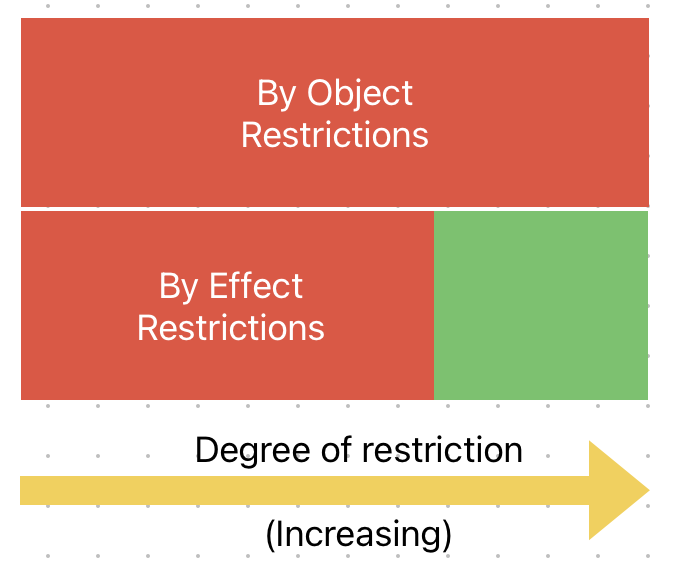
\includegraphics[width=\linewidth]{object_effect_restrictions.png}} 

    \begin{quote}
        «Agreements, decisions and concerted practices caught by Article 101(1) of the Treaty which satisfy the conditions of Article 101(3) of the Treaty shall not be prohibited»
    \end{quote}

    \begin{enumerate}
        \setcounter{enumi}{3}
        \item EU competition law is based on a self-assessment principle. In other terms, parties to an arrangement cannot file it to the EU Commission to obtain a decision declaring that the notified arrangement is lawful such that they can implement it without any fear that at a later time someone will challenge it.
        \item To perform the ex-ante self-assessment the parties must refer to the case-law. In addition, EU Commission facilitates self assessment by issuing regulations, guidelines, notices, etc. covering:
            \begin{enumerate}
                \item general topics (how to determine relevant markets, agreements of minor importance; licensing of intellectual property); 
                \item specific behaviour and practices (cooperation agreements, vertical agreements, etc.), 
                \item or the application of the law in specific sectors (insurance, automotive, etc.).
            \end{enumerate}
        \item Antitrust enforcement in the field of arrangements is an \textit{ex post-facto} enforcement. The Commission may at any time start an investigation \textit{ex officio}, pursuant a complaint, or because of a leniency application. The same applies for private enforcement: a plaintiff claims in a court that an agreement is prohibited and void and/or ask for compensation
        \item In sum, antitrust enforcement follows a typical “stick and carrot” pattern.
            \begin{enumerate}
                \item Clear \& transparent guidance to market agents as to what is and what is not allowed (education); 
                \item Various kind of sanctions to punish wrongdoing and ideally nudge firms to avoid any future violation of the law (punishment, deterrence, and compensation).
                \item Given that full deterrence is impossible (crime always pays!), other tools can be – and in many countries are indeed - used to prevent and/or obstruct the most serious infringements: Leniency, whistle-blowing, and the promotion of compliance programs\sn{\Note{They all influence the very rough enforcement effectiveness index \( EEI = \frac{\# Prohibitions}{\# Violations}\)}}.
            \end{enumerate}
    \end{enumerate}

\section*{Arrangements}

    The constituent elements of the notion of arrangement according to EU competition law are the following ones: 

    \begin{enumerate}
        \item \textbf{Multilateralism} (2 or more subjects involved); 
        \item A \textbf{meeting of minds} between them on what to do/not to do; 
        \item The \textbf{characterisation} of those subjects as “undertakings”.
    \end{enumerate}

    \section{Multilateralism}

        \Definition{An arrangement is the meeting of minds between 2 or more subjects (undertakings/firms).}{Arrangement}

        \begin{enumerate}
            \item If 4 firms agree (in any form) to increase the price of their product, this behaviour can be qualified as an agreement.
            \item On the contrary, if a firm increases the price of its products in a truly autonomous way, this is not an agreement (no meeting of minds with any competitor).
            \item This remains true even if, after the first price increase, other firms in turn follow and increase their price as well. Here, the economic effect is similar to (A); however, since this is the outcome of individual and independent decisions/strategies, antitrust authorities cannot apply Article 101.
        \end{enumerate}

        The EUCJ, in the so-called Sugar case, held that Article 101 TFEU: 

        \begin{quote}
            “does not deprive economic operators of the right to adapt themselves intelligently to the existing and anticipated conduct of their competitors. [...] the fact that a vendor aligns his price on the highest price charged by a competitor is not necessarily evidence of an (arrangement) but may be explained by an attempt to obtain the maximum profit”.
        \end{quote}

        There are many examples of unilateral behaviour that may have an adverse impact on markets and TS, but until very recently couldn't be attacked under Article 101 for lack of multilateralism: Mr. Carlos Tavares, CEO of of Stellantis announces in a public speech that Stellantis is going to increase the price of its cars by 20\%. Obviously, this piece of information may influence competitors of Stellantis and they may eventually increase their prices as well. However, if (and only if) the price announcement was not agreed upon by the parties and/or part of a wider collusive scheme, given the lack of multilateralism Article 101 should not applicable.\sn{\Note{in the U.S. such behaviour is prohibited as an unfair method of competition)}}

    \section{Meeting of Minds}

        \Remark{Article 101 refers to: 
        \begin{enumerate}
            \item «Agreements» 
            \item «Decisions of associations of undertakings»
            \item «Concerted practices»
        \end{enumerate}
        Thus we have three ways of defining what a meeting of minds is:}

\newpage

        \subsection{Agreements}

            EU Tribunal, T-41/96, Bayer (2000):

            \Definition{The concept of agreement: “centres around the existence of a concurrence of wills between at least two parties, the form in which it is manifested being unimportant so long as it constitutes the faithful expression of the parties’ intention”.}{Agreements}

            The notion of agreement within the meaning of art. 101

            \begin{itemize}
                \item A legally enforceable (written or oral) contract, as well as a gentleman’s agreement or a simple understanding, although the latter ones are neither legally binding, nor supported by enforcement procedures;
                \item An individualised or a standard-form contract;
                \item MOUs, draft preliminary agreements, protocols;
                \item Even agreements signed by unauthorised people (if followed by the parties);
            \end{itemize}

            What counts is just a genuine concurrence of wills among the parties; in other words, their meeting of minds, on a certain positive or negative action. This notion of agreement is really broad, so to prevent firms from eluding it.

            \textbf{Therefore}, we have an agreement regardless of the “form” of the “meeting of minds”, i.e. a binding contract or a more subtle or impalpable form of arrangement.

            \Remark{\textbf{Furthermore}, the fact that an undertaking has voluntarily signed it or has been nudged, or even forced into an agreement by other undertakings does not affect the existence of such an agreement. This is a matter of liability / fine calculation.}

            \Example{French Beef: an agreement between French breeders and slaughterers, which required the latter not to import cows from abroad, was deemed to be a prohibited restriction of competition despite the fact that the agreement was reached and implemented by the breeders using physical force: At that time, throughout most of France, groups of farmers illegally stopped lorries in order to check the origin of the meat being transported. In the documents drawn up by the farmers' unions, these illegal interceptions are generally described as "inspections" (contrôles). In addition, slaughterhouses were blockaded by farmers, who prevented any vehicles from entering or leaving the slaughterhouse and/or checked the geographical origin of the meat. These protests and their consequences were widely reported in the press. In most cases, the protest action resulted in the loss of meat which had gone bad after several days of being held up in a blockade, or in meat of non-French origin being burned. Occasionally, the protests resulted in material damage, sometimes on a very substantial scale. For example, on 15 October 2001, farmers ransacked two premises in the department of Ille et Vilaine and destroyed several tonnes of meat.}

            \noindent
            In theory you can break up an arrangement in 3 different phases:

            \begin{enumerate}
                \item A \& B reach an agreement on p (we will increase p by 10\%) (constitutive phase) 
                \item A \& B implement the agreement on p (they will change their price list accordingly) (implementation phase)
                \item Given the agreement, market price will increase by 10\%) (impact or market effect)
            \end{enumerate}

            When analysing an agreement, the focus is primarily on (A). When there is an obvious, extreme, and imminent danger for competition the Commission prohibits the agreement without looking at (B) and (C). In other terms, we look at the capability of restricting competition. Implementation (B) and market impact (C) are still important, though: they influence the level of the fine (seriousness of the infringement; aggravating and mitigating factors).

        \subsection{Decisions of associations of undertakings}

            \textbf{Preamble}: Coordination among firms may be achieved via the medium of trade associations, such as the association of glass producers, the federation of French farmers, the Premier Football League, or the general council of the Dutch Bar. Indeed, AoU may:

            \begin{enumerate}
                \item conceive and promote an illegal agreement – sometimes they are induced to do it by the most powerful firms of the sector\sn{\Note{In some circumstances AoU act as a promoter, in other cases they are only the “veil” under which the real promoters hide}};
                \item practically organise its enforcement; and
                \item control that the firms which are part of the agreement comply with the collusive rules.
            \end{enumerate}

            \Remark{\textbf{How?} Via meetings and exchanges of information among its associates.}

            \textbf{Therefore}, Article 101 directly focuses on the decisions of these trade associations (which, however, are at least indirectly a kind of arrangement between two or more undertakings).

            A decision is any act of the AoU, such as: 

            \begin{itemize}
                \item a deliberation taken by the council/board of the AoU;
                \item a non-binding recommendation adopted by the president of the AoU;
                \item a regulation governing the operations of the AoU;
                \item a code of conduct establishing advertising practices, tariffs, hours of labour and so forth.
            \end{itemize}

        \subsubsection{Who is liable?}

            \begin{enumerate}
                \item All or some members use the AoU merely as a place to conceive and operate the cartel. The AoU is only the locus (it may have been a restaurant, a nice ski resort, etc.) where the parties meet. Here we have an «agreement» between the parties. No active/passive role is played by the AoU. 
                \item Same as a), but the AoU helped with organizing/manage the infringement (gathering information, leading the discussion, solving disputes, etc.). Here, not only the parties, but also the AoU is liable. 
                \item We have a truly AoU decision. The President of an AoU encourages its members to raise prices; the AoU publishes a newsletter urging its members to align to a certain, anti-competitive behavior, etc. The parties did not take part to the decision and/or the discussions leading to the decisions. HERE, the AoU is directly LIABLE for the infringement (and the parties?)
            \end{enumerate}

            \Remark{Under (c) According to Reg. 1/2003, the fine is still 10\% of total turnover. However, turnover in this event is the SUM of each members’ turnover.}

        \subsubsection{Fining an association of undertaking (AoU) in practice.}

            Thus, the fine the AoU may be asked to pay may be very severe. If the AoU is not solvent, it is obliged to call for contributions from its members to cover the amount of the fine. Where such contributions have not been made to the AoU within a fixed time-limit, the EU Commission:

            \begin{enumerate}
                \item may require payment of the fine directly by any of the undertakings whose representatives were members of the decision-making bodies of the AoU. 
                \item if this is still not enough, it may require payment of the balance by any of the members of the AoU which were active on the market on which the infringement occurred.
            \end{enumerate}

            The Commission shall not require payment under a) and b) from undertakings which show that they have not implemented the infringing decision of the AoU, and either were not aware of its existence or have actively distanced themselves from it, before the Commission started investigating the case.

            \Remark{\textbf{Rational of this rule?} To prevent firms to use AoU to escape liability.}

            Granted the very broad scope of the notions of “decisions by association of undertakings” and “agreements”, is there any room for other types of arrangements? Let's move to the concept of \textbf{concerted practice}.

\newpage

    \subsection{Concerted Practice}

            ECJ, 48/69, ICI v. Commission:

            \Definition{A concerted practice is… “a form of coordination between undertakings which, without having reached the stage where an agreement properly so-called has been concluded, knowingly substitutes practical cooperation between them for the risks of competition”}{Concerted Practice}

            A way in which parties knowingly adopt a practice (which does not imply an agreement of what “to do” or “not to do”) which reduces strategic uncertainty in the market, thereby facilitating collusion (we also uses the expression “facilitating practices”). In other words, firms do not agree on a certain variable (such as price, a price increase, etc.), but simply tell each other at what price they will sell their goods in the future. Here, Comp. Authorities can reasonably deduce that the parties’ aim, and reasonable belief is that they will use such information to adapt their future strategies.

            \begin{figure}[h]
                \centering
                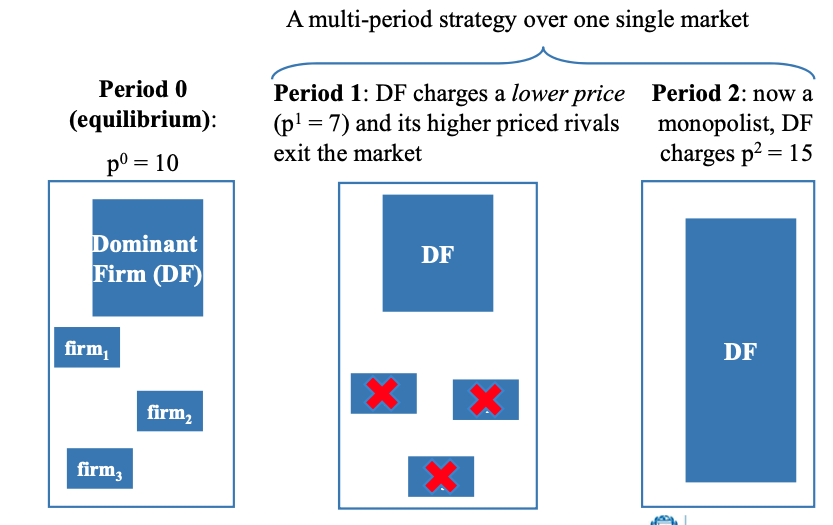
\includegraphics[width=0.85\linewidth]{image.png}
                \caption{Both the boxes represent the building blocks of the notion}
            \end{figure}

            Commission’s Guidelines on the applicability of Article 101 of the Treaty on the Functioning of the European Union to horizontal co-operation agreements, § 63:

            \begin{quote}
                “when a company receives strategic data from a competitor (be it in a meeting, by email, etc.), it will be presumed to have accepted the information and adapted its market conduct accordingly unless it responds with a clear statement that it does not wish to receive such data”
            \end{quote}

            \Remark{\textbf{Result:} No need of bilateral disclosure of information}

            Taking public distance from the exchanged information – i.e. stating that you are not interested in receiving that information – is (almost) the only way out, i.e. the only way to defend a firm from the charge of having been a party in a concerted practice! (other possible way-outs? (A) no info received; (B) Chinese Walls; (C) proof that the information received was completely useless given that your pricing strategies depends only on other variables, etc.). The Commission considers public distance crucial also because it creates distrust!

            \Example{
            Consider the following facts:
            \begin{enumerate}
                \item \textbf{Contacts:} The CEOs of two firms, A and B, share some data about their business strategies … about prices, costs, \textit{et cetera.}
                \item \textbf{Internal use:} Afterwards, the two CEOs use those data to shape and design the strategies of their own firms;
                \item \textbf{Parallel market behaviours:} A and B try to put in practice these new strategies by, for example, increasing their own prices – $P_A$ and $P_B$;
                \item \textbf{Market effects:} The market price $P_{mkt}$ alings to $P_A$ and $P_B$.
            \end{enumerate}
            }

            \Remark{Which, among these events, must occur (and be proved) in order to have a concerted practice? Which of these events are the building blocks of this notion? The first two, granted that the second is presumed}

        \subsubsection{Agreements and concerted practices may be deconstructed in the same way}

            \begin{enumerate}
                \item[a.] \textbf{Constitutive phase} – Meeting of mind (e.g., let’s increase the price; I tell you that I will increase the price, with the presumption that you will take good note of the information received) (1-2).
                \item[b.] \textbf{Implementation} – We take a decision to increase the price, changing our price list (3).
                \item[c.] \textbf{Effects} – We successfully apply the new price list to our customers (4).
            \end{enumerate}
            
            \begin{itemize}
                \item (c) Not necessary.
                \item (b) Not necessary: You may or may not increase the price, or increase it only by a smaller percentage, but… your decision to increase or not the price also depends on the information received.
            \end{itemize}

            \Remark{\textbf{Remember}: Why (a) is sufficient? Given the high moral disvalue of collusion and its harm to society (CS and TS) in the form of a “robbery” to consumers, “prevention is better than cure”.}

            \noindent Implementation and impact are not necessary to find an agreement or concerted practice. However, can a certain market conduct be indicia/evidence of concertation?

            \begin{enumerate}
                \item Parallel conduct (symmetrical and timely increases in prices);
                \item «Strange» behaviour, like rotation in awarding bids, etc.
            \end{enumerate}
            
            \noindent Consider (1). Parallel conduct (e.g., a simultaneous increase in price) may be due to market forces (a reaction to a price increase of an input in perfect competition, oligopolistic interdependence), or it may be the result of a concerted practice.
            
            Thus, in general, parallel behaviour is not enough to prove a restriction of competition. You should find other “external” indicia (e.g., information exchanges, contacts, meetings, or an agreement).
            
            However, when the conduct is irrational, against companies' economic interests (withdrawal from profitable markets or bids), or not justified by the structure of the market, it may represent indicia of concertation.

        \subsubsection{2000 ATM Milano collusion scheme on gasoline sales}

            \begin{itemize}
                \item The public transport company of Milano (ATM) organised a tender to buy «clean gasoline» for its buses. 
                \item Fifteen firms were invited to participate in the tender procedure.
                \item ATM set the following rules of the game: for each year, 12 monthly bidding lots.
                \item Four small firms decided to participate in the tender in a joint venture (JV). Thus, there were 12 participants competing for 12 lots (this is suspicious!).
                \item At least two bidders could produce enough clean gasoline to win all 12 lots, i.e., no capacity constraints (ENI, Tamoil).
            \end{itemize}

        \subsubsection{Concertation in pratice}

            Given the modern formulation of the building blocks of agreements and concerted practices, the enforcers do not distinguish between those practices, i.e., they do not discuss whether a certain behaviour can be categorised as an agreement or a concerted practice.

            \noindent What really counts is the distinction between collusive and non-collusive behaviour.
            
            \noindent \textbf{Commission, PVC (1994):}
            
            \begin{quote}
            ``In the context of a complex infringement which involves many producers seeking over a number of years to regulate the market between them, the Commission cannot be expected to classify the infringement precisely, for each undertaking and for any given moment, as in any event both those forms of infringement are covered by Article (101).''
            \end{quote}
            
            \noindent (When the infringement is long, it may take different forms over time.)

        \subsubsection{Single Overall Agreement}

            Many cartels are complex and of very long duration (some of them lasted dozens of years). Prof. Oindrila De, in Analysis of Cartel Duration: Evidence from EC Prosecuted Cartels, 2010 analyses the life span of cartels convicted by the European Commission between 1990 and 2008. The distribution of cartel life span is right-skewed with a very long tail. The longest lasting cartel in that dataset is the Belgium Architect Association, which lived 36 years. The average mean duration of the cartels is 8.08 years where the median life is 6 and standard deviation is 6.3.

            Over such a long period of time, some firms may be more active than others; some may drop out for a while, and then re-enter the cartel; some can attend a couple of meetings but not others; forms of concertation may change (an agreement, then only information exchanges, then a decision of the trade association where all the members of the cartel belong, etc.).

            If the AAs were to analyze such situation as consisting of several discrete “infringements”, they should launch a bunch of different investigations. However, for some of these practices (the oldest ones), limitation rules prevent the imposition of fines…. (limitation periods/rules, 5 years\sn{\Note{The time limit within which a lawsuit must be brought.}}.

            If, on the contrary, it is possible to categorize this different facts as different tiles of the same mosaic or, in the antitrust gergon a Single Overall Agreement (SOA), only one investigation would be needed, and it is less likely that a limitation problem will arise.

        \subsubsection{T-204/08, Team Relocation (2011)}

            \noindent To have a \textbf{Single Overall Agreement (SOA)}, 3 conditions must be met:

            \begin{enumerate}
                \item The existence of an overall plan pursuing a common objective (e.g., raise the price);
                \item The intentional contribution of each undertaking to the plan; the fact that some members participate less than others or had some reservation about whether to participate, or cheated, does not mean that they are not party to an overall agreement (all the firms participated, even if in different ways, in the plan);
                \item Awareness (presumed or proved) of the offending conduct of the other participants. It is necessary to prove that each undertaking knew, or ought to have known, about the offending conduct of the other members of the cartel (or at least some of the elements of the overall cartel—partial liability).
            \end{enumerate}
            
            \noindent \textbf{Implications:}
            
            \begin{itemize}
                \item Each infringing undertaking is liable for the overall cartel, even though some did not attend every meeting of the cartel, or were not involved in every aspect of its decision-making;
                \item If the various facts can be considered as part of an SOA, then only one fine can be applied (not separate fines). This is important to calculate duration and, also—in a private enforcement action—damages;
                \item The Commission can impose fines in respect of illegal practices that would otherwise be time-barred.
            \end{itemize}
            
\section{Proof of Agreements}

    \begin{enumerate}
        \item[(a)] No problem when the text of the agreement is public, when it is found during a dawn raid, or when it is spontaneously produced by one of the parties.
        \item[(b)] Indeed, if the undertakings are aware of the illegality of the behavior, proof of the agreement is difficult to find because the parties try—and are taught—to conceal all the incriminating evidence. It is also common practice for members of a cartel to camouflage or alter documents to avoid the detection of anti-competitive practices, e.g., by processing agendas or resumes with different content than what was discussed in a meeting; by adopting encryption codes to conceal the names of businesses or employees, or to make unreadable the data and information exchanged; or by providing supporting documents for travel other than the actual motive of travel.
    \end{enumerate}
    
    \noindent Thus, usually, no "smoking gun" is available. It is therefore necessary to understand which elements can indirectly prove the existence of an agreement.

    \subsection{Leniency applicant testimony (Siemens)}

        \noindent A leniency applicant admits the existence of an agreement. The testimonies of business representatives should be considered as particularly reliable (even if indirect) evidence, as they are contrary to the interests of the applicants. But what if they are exaggerating the facts in order to obtain more discounts?

        \noindent \textbf{General Court (GC), Siemens:}
        
        \begin{quote}
        ``As regards the level of credibility to attribute to ABB’s statements, it must be observed that … ABB could reasonably have expected to benefit from the absolute immunity from fines. Therefore, it cannot be ruled out that it might have felt inclined to maximise the significance of the infringing conduct which it was revealing, in order to harm its competitors on the market.
        
        That does not, however, mean that ABB’s statements are to be regarded as devoid of all credibility (…). Indeed, any attempt to mislead the Commission could call into question the sincerity and the completeness of cooperation of the person seeking to benefit, and thereby jeopardise his chances of benefiting fully under the Leniency Notice.
        
        Nonetheless, in so far as those statements from ABB are disputed by other undertakings which are also alleged to have agreed upon the common understanding, they must be supported by other evidence in order to constitute adequate proof of the existence and the scope of the common understanding.''
        \end{quote}

    \subsection{Precise, consistent and reliable indicators}

        In the absence of direct evidence or of convincing confessions, the CJEU, aware of the consequent practical frustration of the aims pursued by antitrust law which would arise from a too strict attitude, considers it sufficient that the EU Commission infers the existence of the cartel indirectly, through “precise, consistent and reliable indicia of all the essential elements of the infringement” (CJEU, C-403-405/04, Sumitomo). However, the EU Commission should collect a set of sufficient and particularly convincing and solid indicia.\sn{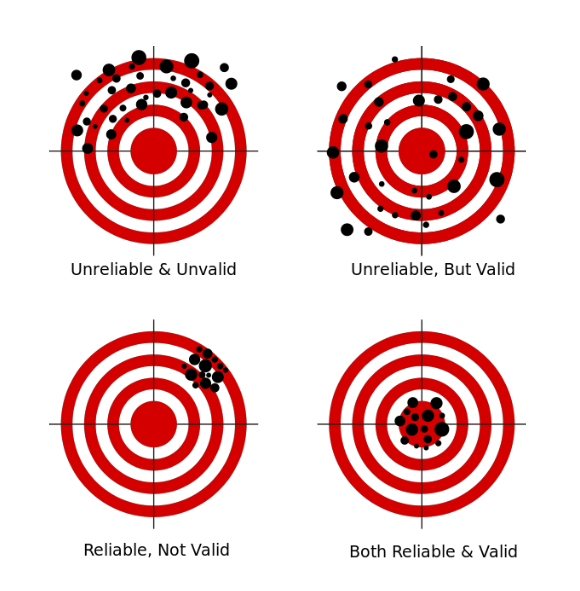
\includegraphics[width=1\linewidth]{reliable_valid_indicia.png}}

        \subsubsection{Different pieces of the puzzle with different evidentiary value}

            Not every indicia has to satisfy the requirement of precision, consistency and reliability in relation to each element of the infringement. It is sufficient that all the indicia, taken as a whole, meet that requirement. This statement is also explained by the notoriety of the antitrust prohibitions against anti-competitive practices, and the resulting secrecy and covert nature and functioning of cartels.

            \newpage

            CJEU, \textit{Sumitomo}, It is normal that anti-competitive practices take place:

            \begin{quote}
                 “in a clandestine fashion, for meetings to be held in secret, and for the associated documentation to be reduced to a minimum. It follows that, even if the Commission discovers evidence explicitly showing unlawful contact between traders, it will normally be only fragmentary and sparse, so that it is often necessary to reconstitute certain details by deduction. Accordingly, in most cases, the existence of an anti-competitive practice or agreement must be inferred from a number of coincidences and indicia which, taken together, may, in the absence of another plausible explanation, constitute evidence of an infringement of the competition rules"
            \end{quote}

        \subsubsection{Indicia, evidence and the congruence of the prosecutorial hypothesis}

            The guiding criterion is that of ``narrative congruence''. The prosecutorial hypothesis supported by several concordant indicia can be confirmed in the decision when it is the only one to give a satisfactory meaning to the 'history' proposed for the reconstruction of the unlawful practice.

            Two different steps are necessary to obtain ``narrative congruence''.
            \begin{enumerate}
                \item Corroboration of the hypothesis, which consists in obtaining information consistent with that used in the inference; and
                \item Cumulative redundancy, which consists in verifying the existence of alternative hypotheses.
            \end{enumerate}
            
            In the absence of direct evidence, therefore, the prosecutorial hypothesis can be accepted \textit{if and only if}:
            \begin{enumerate}[label=\roman*.]
                \item it is the only one capable of justifying and connecting the various elements of the indictment, or at least
                \item it is clearly preferable to any abstractly existing alternative hypothesis.
            \end{enumerate}

    \subsection{Proof of the participation of each undertaking to the agreement}

        Competition Authorities must not only demonstrate the existence of a common understanding, but also identify the undertakings participating in it, albeit with different times, forms, and roles.

        In principle, each of the parties that have signed and/or implemented the agreement is considered as an undertaking participating in the concertation and thus liable for it.
        \begin{enumerate}
            \item We have already seen that if a Single Overall Agreement has been identified, members of the agreement are always liable and the active participation in each of the implementing steps of the “common plan” is irrelevant.
            \item Furthermore, the fact that an undertaking does not adhere to the outcome of meetings cannot deprive it of its full responsibility. The mere fact that the firm did not follow in some circumstances the rules of the cartel could, in fact, derive from temporary internal conflicts or rivalries, or even cheating attempts, but which are perfectly framed in the logic of a concertation.
        
            Furthermore, as already seen, implementation and impact are important factors for the calculation of fines, not for the finding of an infringement.
            \item To demonstrate that an undertaking did not participate in (or abandoned) a collusive agreement, it must prove ``public dissociation''. Dissociation must be expressed firmly and clearly to the other members of the anti-competitive agreement.
        \end{enumerate}

        \subsubsection{Public dissociation/distancing}

            Leaving a meeting is not sufficient, because only through explicit dissociation do the other companies become aware that the competitor believes the conduct is unlawful and does not intend to cooperate to implement it.
        
            This is also because the aim of antitrust enforcers is to break the climate of reciprocal trust between the members of a cartel. Without an active dissociation, the enterprise would give the impression that it supports the agreement and that it will conform to it.
        
            Very strict interpretation: CG, 19-3-2009, \textit{Archer Daniels}: not sufficient to send a letter expressing concern about price discussions, as well as inviting the president of the association to take steps to avoid such anti-competitive practices (no clarification to the other undertakings that it was distancing itself from the hypothesis of such an increase).

        \subsubsection{The nature of the beast}

            Since Art. 101 (and 102) talks about arrangements among 2 or more “undertakings”, EU antitrust enforcers have always struggled with the interpretation of the word “undertaking”.

            \Remark{The issue has always been: \textbf{what is actually an undertaking?}}

            Many and varied answers are given to this question. They have been seriously affected by the specific cases under scrutiny and by some social and economic goals that EU authorities wanted to pursue.\sn{\Note{Functional interpretation of the notion}}

        \subsubsection{Some clear points}

            According to the ECJ:
            \begin{itemize}
                \item To be an undertaking, an entity must be ``engaged in an economic activity, irrespective of its legal status and the way in which it is financed'' -- see \textit{Hofner and Elser v. Macrotron GMbH}, [1991].
                \item An economic activity is any activity consisting in offering goods or services on a given market -- see \textit{Pavlov}, case C-180/98 [2000], § 75.
                \item The various activities carried out by an entity must be considered individually. Even if we consider some of them as ``non-economic activities'', still we can consider the others as economic activities -- see GC, \textit{Selex sistemi Integrati Spa}, [2006] (principle of division).
            \end{itemize}

            \Example{
            A public school might be found not to engage in any economic activity when it provides educational services on a solidarity basis; but it is likely to be deemed an undertaking when, in the evening, it rents out its facilities to a Guitar ``maestro''.
            }

\section{What is (and is not) an undertaking}

    It does not matter whether a firm:
    \begin{enumerate}
        \item is incorporated under a national company law,
        \item has any other legally recognised form,
        \item is owned by a Member State, a Region, or local public body,
        \item is financed with public national or European funds,
        \item is intended to earn profits.
    \end{enumerate}

    \Remark{
    It is enough that the firm is subject to market forces (demand and supply) and carries out its activity with the aim to at least cover its costs with its revenues.
    }

    Entities carrying out activities of pure solidarity are not undertakings, because these are not considered economic activities: no rational agent would ever devote time and resources to them! In the field of social security, the Court has held that certain bodies entrusted with the management of statutory health insurance and old-age insurance schemes pursue an \textbf{exclusively social objective} and do not engage in economic activity. 
    
    The Court has found that to be so in the case of \textbf{sickness funds} which merely apply the law and cannot influence the amount of the contributions, the use of assets and the fixing of the level of benefits. Their activity, based on the principle of national solidarity, is entirely non-profit-making and the benefits paid are statutory benefits bearing no relation to the amount of the contributions (CJEU, \textit{Poucet and Pistre}).

    \begin{itemize}
        \item The notion of undertaking under EU antitrust law is very broad. It encompasses companies, partnerships, agricultural cooperatives, sport associations, and even self-employed people (including performing artists\sn{\Note{This is unless they are employees following the orders/directives of their employers, see later in these notes.}}).
        \item Indeed, natural persons, even members of the professions, can qualify as undertakings. What matters is the economic interest pursued (i.e. whether it is independent or not), not whether the individual is subject to a regulatory body or to a State authorisation.
        \item Thus, architects, engineers, lawyers, a notary public, they all are ``undertakings'' according to EU competition law.
        \item Instead, final consumers never constitute an undertaking (nor an agent operating also on the supply side of the market).
    \end{itemize}

\section{Single Economic Entity (SEE)}

    In \textit{Akzo Nobel}, the ECJ ruled that a SEE consists of:
    \begin{quote}
    ``a unitary organisation of personnel, tangible and intangible elements, which pursue a specific economic aim on a long-term basis.''
    \end{quote}
    
    Furthermore, the concept of an undertaking must be understood as designating an economic unit even if in law that economic unit consists of several persons, natural or legal (\textit{Confederación Española de Empresarios de Estaciones de Servicio}, §40).
    
    In this scenario, there is no independence, no autonomous or independent parties that can determine their course of action in the market.
    
    Consequently, there can be no restriction of (a non-existing) competition between a parent company and its subsidiaries or between several subsidiaries of the same parent company, given that they are part of the same undertaking.

        \subsubsection{Test of control/decisive influence \textit{in concreto}}

            The test is whether the parent company "P" (i) \textit{can} and (ii) \textit{does in fact} exercise decisive influence\sn{\Note{Decisive influence, or better, effective control, must be not only a prospect, a possibility, or an opportunity; on the contrary, it must be concrete, real, and tangible.}} over the subsidiary ``S'', with the result that the latter does not enjoy ``real autonomy'' in determining its commercial policy on the market.
            
            For these purposes, it is necessary to examine all the relevant factors relating to the economic, organisational, and legal links which tie the subsidiary to the parent company\sn{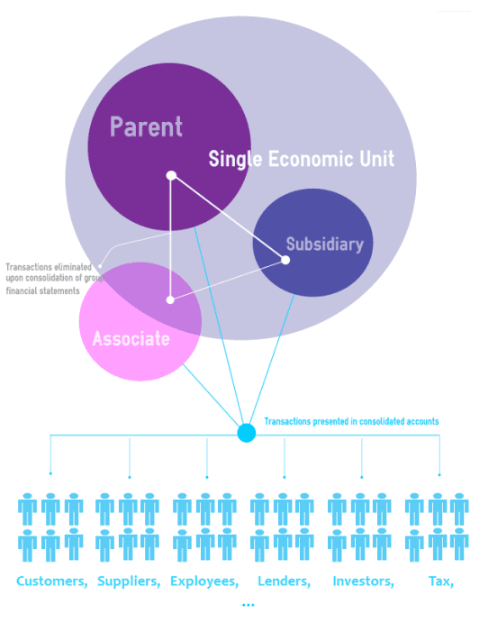
\includegraphics[width=1\linewidth]{SEE.png}}. When the parent company has a 100\% (NOW: almost 100\%) shareholding (and now, after ECJ in 2020 \textit{Goldman Sachs}, voting rights) in a subsidiary, there is a rebuttable presumption that the parent does in fact exercise such influence\sn{\Note{In practice, it is almost impossible to rebut it.}}.

    \subsection{Consequences}

        The application of the SEE principle has 2 fundamental consequences for the entities concerned, the first one “positive”, and the second one “negative”.
        
        \textbf{The positive one}: an agreement between a parent and a closely (effectively) controlled subsidiary, which are thus deemed to form a SEE, does not fall within Article 101. P is free to give S directives as to investments, production, marketing strategies, etc. The two firms are in fact considered one and the same entity (and an entity cannot conclude an \textbf{anticompetitive} agreement with itself).
        
        In sum, no intra-enterprise conspiracy (within the SEE) is possible.
        
        \textbf{The negative one}: If the subsidiary Sub1 infringes Article 101/102 and is deemed to form a SEE with its parent P, then:
        \begin{enumerate}[label=(\alph*)]
            \item The investigation (formally) will involve both Sub1 and its parent company P, and the decision is addressed to both Sub1 and P;
            \item P is jointly and severally liable with Sub1 for any fine imposed on its subsidiary;
            \item The maximum fine (10\% of the infringer’s worldwide turnover) refers to the turnover of the entire SEE (i.e., P group’s turnover which may be vastly greater than Sub1's turnover);
            \item The level of the fine depends on many factors, among which recidivism. Again, recidivism is referred to the SEE, which means that the fine on Sub1 may be higher because either P or another of its subsidiaries (Sub2) had committed similar infringements in the past. Also, the dissuasive factor must be referred to the SEE.
        \end{enumerate}
        
        \Remark{These consequences apply even if P did not incentivize/instigate or at least knew about the infringement.}
        
        From a public enforcement perspective, the SEE doctrine is very important because:
        \begin{itemize}
            \item For serious anticompetitive behaviour, fines will be higher (i.e. more deterrent), given the increase of the turnover to which the legal maximum 10\% percentage refers;
            \item Fines’ collection will be more likely (if Sub1 is not able to pay, the fine can be collected from P, which is obliged to pay the full amount of the fine because of the joint and several liability rule);
            \item Attributing liability to P can nudge its board of directors to take responsibility for monitoring and eradicating anticompetitive behaviour within the entire group (SEE), for example, by imposing on all subsidiaries to adopt effective antitrust compliance programs;
            \item It limits risk allocation techniques by multinationals to subsidiaries to avoid heavy fines.
        \end{itemize}

        \subsubsection{Internal and external boundaries of the notion of undertaking}

            An undertaking is not (always) a rational atomistic agent; it is an organisation of different factors, whose strategies are decided and supervised by managers (and directors) and carried out by employees and external agents.

            \Remark{Who is liable when the behaviour has been carried out by an employee, or an agent of a firm?}

\section{Employees and Undertaking}

        \subsubsection{1. Actions of employees are attributable to their employer undertaking}

            \Example{ECJ C-542/14, \textit{SIA ‘VM Remonts’}: An employee performs his/her duties for and under the direction of the undertaking for which he/she works and, thus, is considered to be incorporated into the economic unit comprised by that undertaking. }
            
            For the purposes of a finding of infringement of EU competition law, any anti-competitive conduct on the part of an employee is thus attributable to the undertaking to which he/she belongs, and that undertaking is, as a matter of principle, held liable for that conduct.
    
        \subsubsection{2. While employees must have a mandate to represent the firm, the form of the mandate does not count (and mandate may be inferred by the undertaking’s behaviour).}

            \Example{ECJ, \textit{Protimonopolný úrad Slovenskej republiky V Slovenská sporiteľňa a.s.}: It is not necessary to show that the employee had a specific mandate to participate in the anti-competitive behavior when the undertaking has not distanced itself from the conduct of that employee and when, at the same time, the agreement has been implemented.}
        
            As the Commission pointed out, participation in anticompetitive agreements is often clandestine and is not governed by any formal rules. It is rarely the case that an undertaking’s representative attends a meeting with a mandate to commit an infringement.
    
        \subsubsection{3. It is irrelevant whether top managers, directors, or partners took part or had knowledge of the anti-competitive practice.}

            \Example{ECJ, \textit{SA Musique Diffusion française} (1983): The Court observed that, for Article 101 to apply, it is not necessary for an action by, or even knowledge on the part of, the partners or principal managers of the undertaking concerned.}
    
        \subsubsection{4. It is irrelevant that employees acted differently from any directive or instruction received by the undertaking and its managers (at least when analysing the existence of an agreement).}

            Regulation 1/2003 allows the Commission to fine undertakings when either intentionally or negligently they infringe Articles 101 and 102. Thus, an undertaking is also liable for \textit{culpa in eligendo}\sn{\Note{Fault in selecting}} and \textit{culpa in vigilando}\sn{\Note{Fault in supervising}} for the acts of its employees.

\section{Vertical Agreements \& Agency Contracts}

        Agency contracts are commonly used for the sale of goods and services. An agent is a legal or natural person who negotiates contracts with third parties on behalf of its principal. Once the contract is concluded, the agent drops out, with the performance of the contract left to the principal and/or third party.

        Article 101 does not apply to agency contracts (between an agent and its principal) when it can be shown that there is an absence of financial/commercial risk on the part of the agent, who did not take title on the goods being traded.\sn{\Note{This was and still is quite common for mono-brand car dealers. The sale is signed on the behalf of the car producer}}
        
        \textbf{Very important issue!}
        \begin{itemize}
            \item If a principal ``P'' establishes the price at which his agent ``A'' must sell a good to the final customers, or limits its ability to sell to non-residents, or the use of the internet to promote sales, is this behaviour prohibited according to Article 101?
            \item If the agent ``A'' colludes on sharing markets with another agent, is this an agreement between these two agents, or does it also necessarily involve their principals?
        \end{itemize} 

\section{Agency agreements}

    \subsection{Principles}

        An agreement is an ``agency agreement'' where property in the contract goods bought or sold does not vest in the agent, and ``A'', \textit{inter alia}:
        \begin{enumerate}
            \item does not contribute to the costs relating to the supply/purchase of the contract goods or services, including the costs of transporting the goods;
            \item does not maintain at its own cost or risk stocks of the contract goods, including the costs of financing the stocks and the costs of loss of stocks;
            \item does not undertake responsibility towards third parties for damage caused by the product sold (product liability);
            \item does not take responsibility for customers' non-performance of the contract, with the exception of the loss of the agent's commission, unless the ``A'' is liable for fault;
            \item is not, directly or indirectly, obliged to invest in sales promotion, such as contributions to the advertising budgets of the principal;
            \item does not make market-specific investments in equipment, premises, or training of personnel.
        \end{enumerate}

    \subsection{Antitrust Implications}

        These principles are fundamental to allocate liability for a certain behaviour. If ``P'' bears all the commercial and financial risks related to the selling and purchasing of the contract goods and services, all obligations imposed on the agent ``A'' in relation to the contracts concluded and/or negotiated on behalf of P fall outside of Article 101.

        P imposes on A to sell its cell phones only in Rome at the price ``x''.
        \begin{itemize}
            \item \textbf{A is a ``proper'' agent of P:}
            \begin{itemize}
                \item Therefore, no infringement of Article 101.
                \item However, if you consider P and A as a ``one and single'' firm, it is possible to challenge P’s directives to A and their execution under Article 102 (IFF P holds a dominant position and the price x is considered excessive).
            \end{itemize}
            
            \item \textbf{A is independent from P:}
            \begin{itemize}
                \item Article 101 can be applied.
            \end{itemize}
        \end{itemize}

        \subsubsection{The agency principle can be generalised to any external agent, like service providers, dealers, etc., working for the undertaking}

            To gain market power in France, VW Germany is willing to sell its VW Golf cars throughout France at only €10,000. The offer is intended to be limited to the French territory. Thus, VW asks its French dealer (FVW) to refrain from selling VW Golf cars to non-French citizens.

            Is this behaviour anti-competitive?
            
            The answer depends on the relationship between FVW and VW.
            \begin{enumerate}[label=\alph*.]
                \item If FVW, although independent from a legal standpoint, does not bear any commercial \& financial risks related to the selling and purchasing of Golf cars in France, then FVW ``belongs'' to the same SEE of VW. They are not competitors and, thus, no restriction of competition is possible. If ever, the behaviour of (VW+FVW) may be scrutinised under Article 102 (iff VW is dominant).
                
                \item If, on the contrary, FVW bears at least some commercial \& financial risks, then it must be considered as an independent entity. Therefore, the vertical agreement concerning the export ban is caught by Article 101 and forbidden if capable of determining a restriction of competition.
            \end{enumerate}

        \subsubsection{A last point}

            If A is not independent from P, also the negative consequences of the SEE doctrine apply. Thus, P will be liable also in case of an agreement between A and a third party (TP).

            If VWF agrees with Stellantis to share the French market geographically, VW will be liable for the agreement together with VWF (and of course Stellantis).
            
            \[
            VW \quad \longleftrightarrow \quad VWF \quad \longleftrightarrow \quad Stellantis
            \]
            
            Thus, the fine’s cap will be measured on VW group global turnover, VW will be jointly \& severally liable for the payment of the fine, and recidivism and the deterrent factor will be determined by taking into account VW as a group.
            